%
% TU/e Style Master Thesis template for LaTeX
%
% Public version 1.0
%
% THIS IS THE MAIN FILE (i.e. compile this file, compiling the others directly won't work)%
\documentclass[a4paper,10pt,twoside]{report}

%all the other includes etc. are done in the report.sty file.
\usepackage{report}
\usepackage{amsmath}
\usepackage{amssymb}
\usepackage{enumitem}

\usepackage{svg}
\usepackage{tabularx}
\usepackage{tikz}

%
% These commands need to be defined in order to produce a correct and personalized document
%
\newcommand{\coursecode}{2IS55}
\newcommand{\coursename}{Software Evolution}
\newcommand{\shortdoctitle}{\coursecode - \coursename}
\newcommand{\doctitle}{\coursecode\hspace{2mm}-\hspace{2mm}\coursename}
\newcommand\NextYear{\advance\year by 1 \the\year\advance\year by -1}
\newcommand{\docsubtitle}{Assignment 2 (\the\year\hspace{2mm}-\hspace{2mm}\NextYear) }

\newcommand{\me}{Luuk van Hulten (0720248) \\ Nanne Wielinga (0852473)}
\newcommand{\keywords}{\coursecode, \coursename}
\newcommand{\version}{Version 1.0}
\newcommand{\monthYear}{ \today }

%Be sure to use all the titles for your committee members!!! (their names show up on the very first page!)
%\newcommand{\firstCommitteeMember}{Your First Committee Member}
%\newcommand{\secondCommitteeMember}{Your second Committee Member, usually the daily supervisor}
%\newcommand{\thirdCommitteeMember}{Your Third Committee Member, usually the external member}

\author{\me}

%
% PDF settings
%
\hypersetup
{
    pdfauthor={\me},
    pdftitle={\shortdoctitle},
    pdfsubject={\doctitle},
    pdfkeywords={\keywords}
}

\begin{document}

%use this include for PDF and distribution versions
\pagenumbering{roman}
\include{titlepage}

\normalsize

\tableofcontents

\setcounter{page}{2}
\pagenumbering{arabic}


\chapter{Introduction}\label{chapter:Introduction}
The assignment is divided in several tasks. The first task is to build a tool chain for extracting information from a Java program. The tool should extract at least the following information: class names, (static) fields, method signatures, associations, generalisations, realisations and dependencies (defined in Table 3.1 of the book by Tonella and Potrich). The tool chain has to be build using Rascal. Rascal is a domain specific language for source code analysis and manipulation.

The second part is the architecture reconstruction. From the extracted information a class diagram has to be reconstructed. In this diagram there must be a taken care of declared vs. actual types and containers. This diagram has to be visualized.

Finally the tool chain has to be applied on two projects eLib and two versions of the CyberNeko HTML Parser. The acquired results has to be discussed and described in this report.

\section*{Purpose of the assignment}
The purpose of the assignment is identifying interrelations and components of an existing system. Good documentation of the system is required for cost effectively maintenance and modification of a system. Since the documentation of a system can be lacking or outdated, due to the evolution of a system. It is convenient to have tools that extract this information from the existing software (reverse engineering) and generate the documentation like class and flow diagrams directly from the code base. 

\chapter{Input and Output Language}\label{chapter:Input and Output Language}
In this section the input and output languages of the tool is discussed. For each feature it is indicated if it's supported, partly supported or unsupported.

\section{Input}
Many java features are supported by rascal. The following standard functionality is supported by the tool chain: class names, (static) fields, method signatures. Since this information indicates the structure of the classes.
Also associations, generalisations, realisations and
dependencies are supported. Using this information the relations between classes can be extracted. These relations can be used to identify packages, redundant classes and so on.

\subsection*{Inner classes}
Inner classes are classes that are contained within an other class. Inner classes are partly supported since they will be identified as normal classes by the tool. However by doing so the inner class access modifiers is lost.

\subsection*{Generics}
A generic type is a generic class or interface that is parameterized over types.
Are generic types supported?

\newpage

\section{Output}
The output language of the tool is a class diagram conform UML v2.0. The class diagram is generated using the graphviz dot language. We chose to export the class diagram as an svg image since this appeared to support more functionality like underlining and didn't want the visual component to be the bottleneck of the tool.

\subsection*{Packages}
A package is a mechanism for organizing classes into namespaces. Packages are often used in modular programming.  Programmers also typically use packages to organize classes belonging to the same category or providing similar functionality. In the tool packages are supported. The support for packages is added since in larger projects these packages give a better overview of the project.

\subsection*{Named association}
In the tool chain we did not support named associations since this information is not explicit contained within the JAVA language. Hence named associations could only be implied by variable/method names. This makes the functionality unreliable between different projects and why it's better not to support it. However these patterns can still be observed from the class diagram.

\subsection*{Multiplicity}
Multiplicity is also not supported by the application. For multiplicity support the control flow of the application has to be known. This control flow can only observed while running the application.



\chapter{The tool chain}\label{chapter:The tool chain}
The tool is build using rascal. The tool is build under the assumption that the library are functionally correctly under normal usage.

\section*{Abstract syntax tree}
The abstract syntax tree contains information about all types contained in the project. The information is presented as a tree with nodes and children. Using this abstract syntax tree all variable and return types can be extracted. These are then displayed in the class diagram.

\section*{M3 Model}
The M3 model is a wrapper around the abstract syntax tree. Using the m3 all information about classes like class names, methods, etc can be acquired. This information is presented as a set of functions with annotations. The M3 contains the same information as the abstract syntax tree however class information can easier be deduced from the M3.

\section*{Object Flow Diagram}
An object flow is a path along objects of data that gets passed. The object flow is represented as a relation between object calls, assigns and data. The dependencies between object are deduced from the object flow graph.

\begin{figure}[h!]
  \begin{center}
    \includegraphics[width=0.48\textwidth]{figures/easy-workflow.png}
  \end{center}
  \caption{Extract-Analyze-Synthesize (EASY) paradigm}
\end{figure}

\section*{Visualization}
All the acquired information is used to generate a dot file. The dot file contains the class information added with graphical styles. Using graphviz the class diagram can be generated from the dot file.

\section*{Usage}
The tool chain can be used to reverse engineer and generate the documentation like class and flow diagrams directly from java programs. The tool works best on small to medium size projects, since the visualization of class diagram in larger projects should be partitioned in smaller sub diagrams. This functionality is not supported in the current version of the tool. 

\chapter{Apply the tool chain}\label{chapter:Apply the tool chain}
\section{eLib}
The class diagram below is extracted using the tool. Present the Object Flow Graphs required to construct the diagram. Evaluate the precision of the tool developed, its performance and visual quality of the class diagram produced.
 
\begin{figure}[h!]
  \begin{center}
    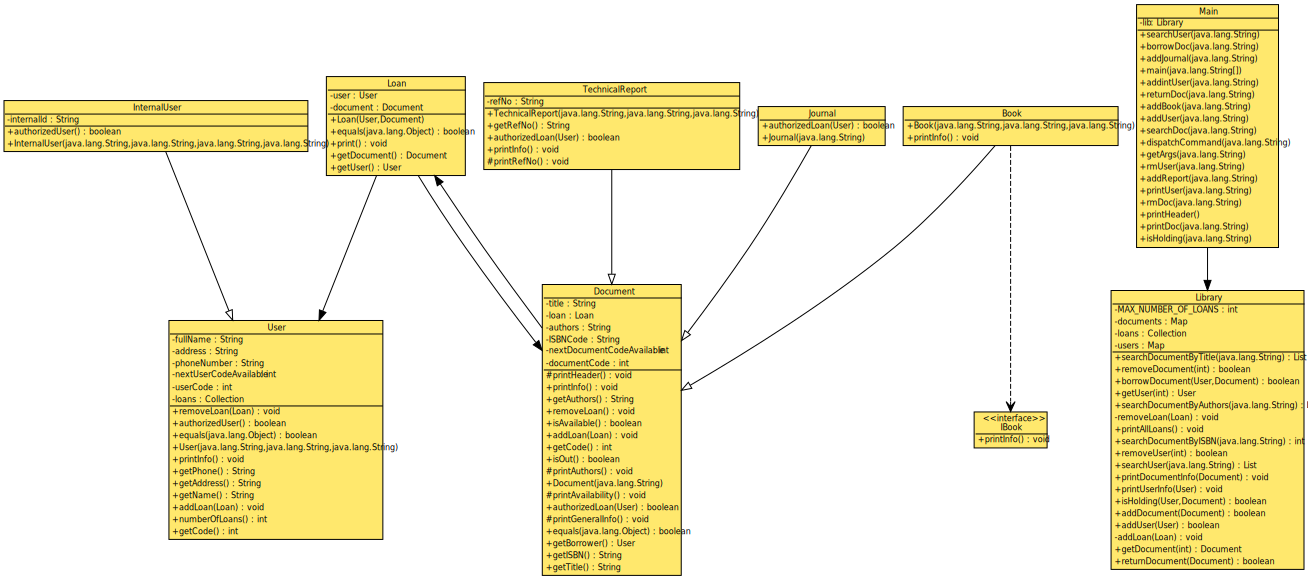
\includegraphics[width=1.0\textwidth]{figures/eLib.png}
  \end{center}
  \caption{eLib class diagram}
\end{figure} 

\subsection{Evaluation}

Evaluate the precision of the tool developed, its performance and visual quality of the class diagram produced. The source code of the eLib benchmark can be downloaded from http://www.win.tue.nl/~aserebre/2IS55/2011-2012/eLib.zip

\section{CyberNeko HTML Parser}

\subsection{Evaluation}

\chapter{Discussion}\label{chapter:Discussion}
\input{chapters/discussion}

\chapter{Conclusion}\label{chapter:Conclusion}
\input{chapters/conclusion}

\end{document}
